% !TEX root = ../main.tex
\section{Ejercicio propuesto 2: pruebas diferenciales y análisis experimental}

\subsection{Metodología de medición y diseño experimental}
Para evaluar la convolución directa, la FFT compleja (recursiva e iterativa) y la NTT modular, implementamos el siguiente protocolo de medición experimental:
\begin{enumerate}
    \item \textbf{Aislamiento temporal estricto:} Pregeneramos todas las entradas en memoria antes de activar el cronómetro de alta resolución \texttt{perf\_counter\_ns()}. La ventana de medición contiene exclusivamente el algoritmo de multiplicación; excluimos la generación de datos, la validación con oráculos, el conteo de operaciones y las operaciones de entrada/salida a disco.
    \item \textbf{Repeticiones y estadística:} Ejecutamos cada combinación de tamaño y método un mínimo de 10 repeticiones independientes. Calculamos el tiempo mínimo, la mediana y el máximo, adoptando la mediana como métrica central por su robustez frente al planificador del sistema operativo.
    \item \textbf{Gestión de memoria y mutabilidad:} Dado que \texttt{fft\_iterative} opera in-place, generamos una copia limpia de los vectores en cada repetición para evitar mediciones sobre arreglos previamente alterados.
    \item \textbf{Rango evaluado:} Medimos potencias de dos $n = 2^k$ con $k \in \{3, 4, \dots, 14\}$ ($8 \le n \le 16\,384$). La convolución directa la evaluamos hasta $n = 2048$ para evitar tiempos prohibitivos de ejecución.
\end{enumerate}

\subsection{Escenario A: Validación diferencial y oráculos de referencia}
Contrastamos la corrección de las cuatro rutas algorítmicas frente a los oráculos exactos sobre tres rangos de coeficientes: pequeños ($[-10, 10]$), medianos ($[-1000, 1000]$) y de gran magnitud ($[0, p-1]$ con $p = 998244353$). La Tabla \ref{tab:manuales} resume los casos manuales y de frontera.

Las Tablas \ref{tab:validacion_fft} y \ref{tab:validacion_ntt} demuestran la fidelidad de la transformación y recuperación directa/inversa (roundtrip). La NTT en $\mathbb{F}_p$ recuperó con exactitud absoluta los vectores de prueba módulo $p$. Por su parte, la FFT de doble precisión exhibió diferencias del orden de $10^{-15}$ a $10^{-14}$ frente a la referencia entera en rangos acotados, coincidiendo de forma idéntica en sus versiones recursiva e iterativa. La Tabla \ref{tab:modulos_raices} documenta la correspondencia de raíces y generadores según la divisibilidad $N \mid (p-1)$.

\begin{table}[htbp]\centering\small
\caption{Casos manuales (coeficientes en orden ascendente)}
\label{tab:manuales}
\begin{tabular}{rrrr}\toprule
Caso & $a$ & $b$ & $c$ \\
\midrule
0 & [] & [1, 2] & [] \\
1 & [0] & [0] & [0] \\
2 & [3] & [-2] & [-6] \\
3 & [1, 2, 3] & [4, 5] & [4, 13, 22, 15] \\
4 & [1, -1] & [1, 1] & [1, 0, -1] \\
5 & [1, 0, 0, 1] & [1, 1] & [1, 1, 0, 1, 1] \\
\bottomrule\end{tabular}\end{table}

\begin{table}[htbp]\centering\small
\caption{Transformadas directas/inversas y diferencia FFT recursiva/iterativa}
\label{tab:validacion_fft}
\begin{tabular}{rrrr}\toprule
$n$ & Error FFT/IFFT & Error iterativa & Diferencia FFT \\
\midrule
8 & 1.9e-15 & 1.9e-15 & 0 \\
16 & 3.9e-15 & 3.9e-15 & 0 \\
32 & 3.9e-15 & 3.9e-15 & 0 \\
64 & 1.5e-14 & 1.5e-14 & 0 \\
128 & 2.5e-14 & 2.5e-14 & 0 \\
\bottomrule\end{tabular}\end{table}

\begin{table}[htbp]\centering\small
\caption{NTT/INTT: recuperación exacta módulo $998244353$}
\label{tab:validacion_ntt}
\begin{tabular}{rrr}\toprule
$n$ & Raíz & Recupera módulo $p$ \\
\midrule
8 & 372528824 & sí \\
16 & 929031873 & sí \\
32 & 452798380 & sí \\
64 & 922799308 & sí \\
128 & 781712469 & sí \\
\bottomrule\end{tabular}\end{table}

\begin{table}[htbp]\centering\small
\caption{Primos, generadores, raíces y longitudes NTT seleccionadas}
\label{tab:modulos_raices}
\begin{tabular}{rrrrr}\toprule
$p$ & Generador & $N$ & $\omega_N$ & $N_{max}$ \\
\midrule
17 & 3 & 1 & 1 & 16 \\
17 & 3 & 2 & 16 & 16 \\
17 & 3 & 4 & 13 & 16 \\
17 & 3 & 8 & 9 & 16 \\
17 & 3 & 16 & 3 & 16 \\
998244353 & 3 & 1 & 1 & 8388608 \\
998244353 & 3 & 2 & 998244352 & 8388608 \\
998244353 & 3 & 4 & 911660635 & 8388608 \\
998244353 & 3 & 8 & 372528824 & 8388608 \\
998244353 & 3 & 16 & 929031873 & 8388608 \\
998244353 & 3 & 32768 & 968855178 & 8388608 \\
998244353 & 3 & 8388608 & 15311432 & 8388608 \\
\bottomrule\end{tabular}\end{table}

\begin{table}[htbp]\centering\small
\caption{Tiempo mediano en ms, 10 repeticiones o más; --: no medido}
\label{tab:tiempos}
\begin{tabular}{rrrrr}\toprule
$n$ & Directa & FFT rec. & FFT iter. & NTT \\
\midrule
8 & 0.012 & 0.129 & 0.090 & 0.131 \\
16 & 0.042 & 0.265 & 0.193 & 0.249 \\
32 & 0.163 & 0.567 & 0.417 & 0.530 \\
64 & 0.648 & 1.219 & 0.916 & 1.143 \\
128 & 2.834 & 2.582 & 2.017 & 2.550 \\
256 & 11.847 & 5.523 & 4.744 & 6.190 \\
512 & 54.738 & 13.458 & 11.515 & 15.482 \\
1024 & 226.228 & 25.252 & 24.851 & 32.558 \\
2048 & 1066.722 & 63.056 & 61.618 & 80.149 \\
4096 & -- & 132.488 & 141.477 & 175.311 \\
8192 & -- & 136.133 & 190.992 & 364.137 \\
16384 & -- & 563.116 & 652.601 & 907.830 \\
\bottomrule\end{tabular}\end{table}

\begin{table}[htbp]\centering\small
\caption{Operaciones ejecutadas en multiplicación; cada mariposa incluye 2 sumas y 2 productos}
\label{tab:operaciones}
\begin{tabular}{rrrrr}\toprule
$n$ & Productos directa & Mariposas FFT & Mariposas NTT & Etapas \\
\midrule
8 & 64 & 96 & 96 & 12 \\
16 & 256 & 240 & 240 & 15 \\
32 & 1024 & 576 & 576 & 18 \\
64 & 4096 & 1344 & 1344 & 21 \\
128 & 16384 & 3072 & 3072 & 24 \\
256 & 65536 & 6912 & 6912 & 27 \\
512 & 262144 & 15360 & 15360 & 30 \\
1024 & 1048576 & 33792 & 33792 & 33 \\
2048 & 4194304 & 73728 & 73728 & 36 \\
4096 & -- & 159744 & 159744 & 39 \\
8192 & -- & 344064 & 344064 & 42 \\
16384 & -- & 737280 & 737280 & 45 \\
\bottomrule\end{tabular}\end{table}

\begin{table}[htbp]\centering\small
\caption{Error FFT antes de redondear (n=1024)}
\label{tab:error}
\begin{tabular}{rrrrr}\toprule
Magnitud & Método & Error real & Error imaginario & Fallos \\
\midrule
10 & rec. & 5.4e-11 & 4.3e-11 & 0 \\
10 & iter. & 5.4e-11 & 4.3e-11 & 0 \\
1000 & rec. & 4.3e-07 & 3.3e-07 & 0 \\
1000 & iter. & 4.3e-07 & 3.3e-07 & 0 \\
100000 & rec. & 0.0041 & 0.0034 & 0 \\
100000 & iter. & 0.0041 & 0.0034 & 0 \\
1000000000 & rec. & 4.6e+05 & 3.6e+05 & 2047 \\
1000000000 & iter. & 4.6e+05 & 3.6e+05 & 2047 \\
\bottomrule\end{tabular}\end{table}

\begin{table}[htbp]\centering\small
\caption{Primer tamaño medido que supera a la convolución directa}
\label{tab:puntos_cruce}
\begin{tabular}{rrr}\toprule
Método & $n$ de cruce & Directa medida hasta \\
\midrule
fft\_recursiva & 128 & 2048 \\
fft\_iterativa & 128 & 2048 \\
ntt & 128 & 2048 \\
\bottomrule\end{tabular}\end{table}


\noindent En nuestro análisis diferencial realizamos 60 comparaciones en el Escenario A; identificamos 10 discrepancias en el rango $[0,p-1]$ con FFT de doble precisión debido a la saturación de la mantisa de 53 bits. Estas discrepancias quedaron registradas en \path{python/results/discrepancias.csv}. Por su parte, la NTT coincidió exactamente módulo $p$ en la totalidad de los casos.\par


\noindent Identificamos que el primer fallo de redondeo en la FFT ocurrió en $n=8$, magnitud máxima 1000000000, semilla 1020360906, método recursive, índice 0: referencia entera -340733537975249223 frente al valor redondeado -340733537975249152. Los vectores de prueba se registran en \path{python/results/primer_fallo_fft.csv}.\par


\subsection{Escenario B: Complejidad temporal, operaciones y puntos de cruce}
La Tabla \ref{tab:tiempos} y la Figura \ref{fig:tiempo} ilustran la evolución del costo temporal empírico en función del tamaño de entrada $n$. Confirmamos la transición asintótica: la convolución directa crece a una tasa cuadrática $\Theta(n^2)$, requiriendo más de un segundo para $n = 2048$, mientras que FFT recursiva, FFT iterativa y NTT exhiben un crecimiento cuasilineal $\Theta(n \log_2 n)$.

\begin{figure}[H]\centering
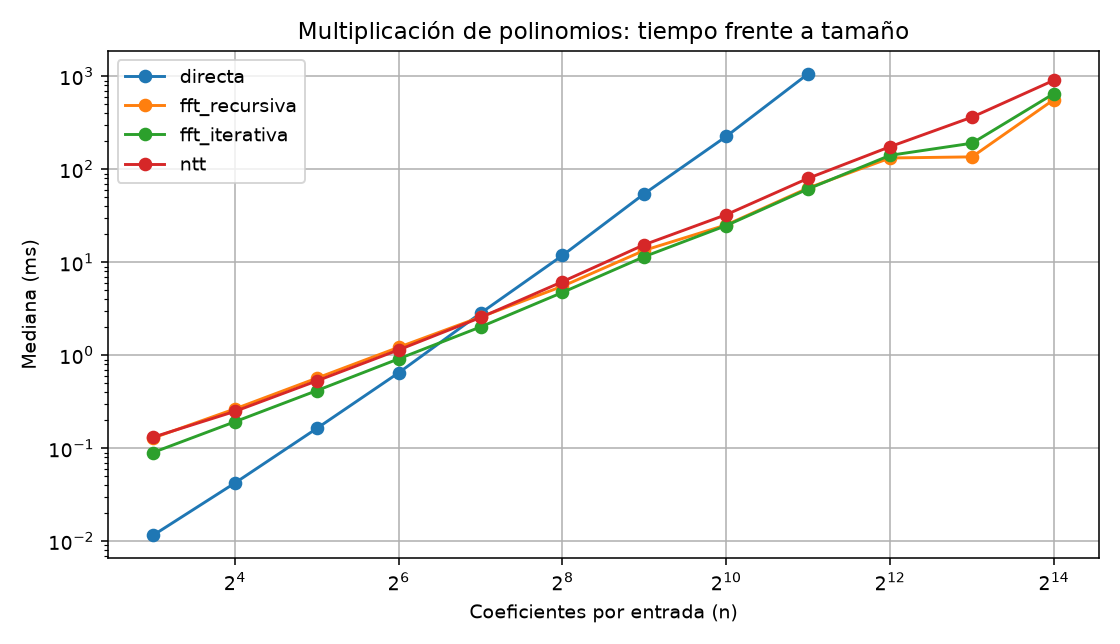
\includegraphics[width=.88\textwidth]{fig1_tiempo_vs_n.png}
\caption{Tiempo mediano de ejecución (ms) frente al tamaño del polinomio $n$ en escala logarítmica. La convolución directa se interrumpe en $n=2048$ por costo cuadrático.}\label{fig:tiempo}
\end{figure}

\begin{figure}[H]\centering
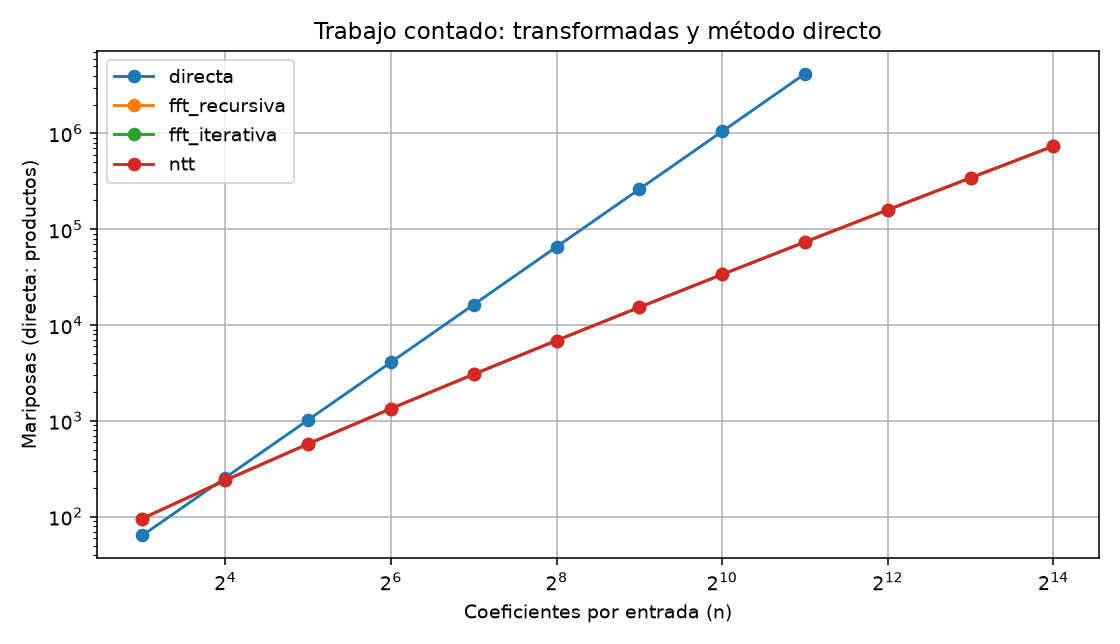
\includegraphics[width=.88\textwidth]{fig2_operaciones_vs_n.png}
\caption{Número de operaciones fundamentales ejecutadas frente a $n$: multiplicaciones escalares directas frente a mariposas radix-2 de FFT y NTT.}\label{fig:operaciones}
\end{figure}

En la Figura \ref{fig:operaciones} contrastamos el número real de mariposas ejecutadas por las transformadas rápidas ($3 \cdot \frac{N}{2} \log_2 N$) frente a las $n^2$ multiplicaciones de la convolución directa:
\begin{itemize}
    \item Para tamaños pequeños ($n \le 64$), la convolución directa es superior en tiempo de reloj real. Aunque su orden asintótico es $\Theta(n^2)$, su constante oculta es mínima: se reduce a bucles nativos sin inicialización de listas auxiliares ni cálculos trigonométricos.
    \item El \textbf{punto de cruce} (crossover point) ocurre a partir de $n = 128$, tamaño en el cual tanto la FFT iterativa (2.017 ms frente a 2.834 ms directa) como la FFT recursiva (2.582 ms) y la NTT (2.550 ms) superan a la convolución tradicional. Para $n = 2048$, las transformadas rápidas son más de 16 veces más veloces que la convolución directa.
    \item Entre FFT iterativa y recursiva, la versión iterativa ofrece una ventaja de tiempo en tamaños pequeños y medianos ($n \le 2048$) al evitar las llamadas recursivas y la asignación de memoria dinámica de Python.
\end{itemize}

\subsection{Escenario C: Precisión numérica, error de redondeo y primer fallo}
La Tabla \ref{tab:error} y la Figura \ref{fig:error} presentan el error absoluto máximo de la parte real $\max |\operatorname{Re}(\tilde{c}_k) - c_k|$ y de la parte imaginaria $\max |\operatorname{Im}(\tilde{c}_k)|$ antes del redondeo entero.

\begin{figure}[H]\centering
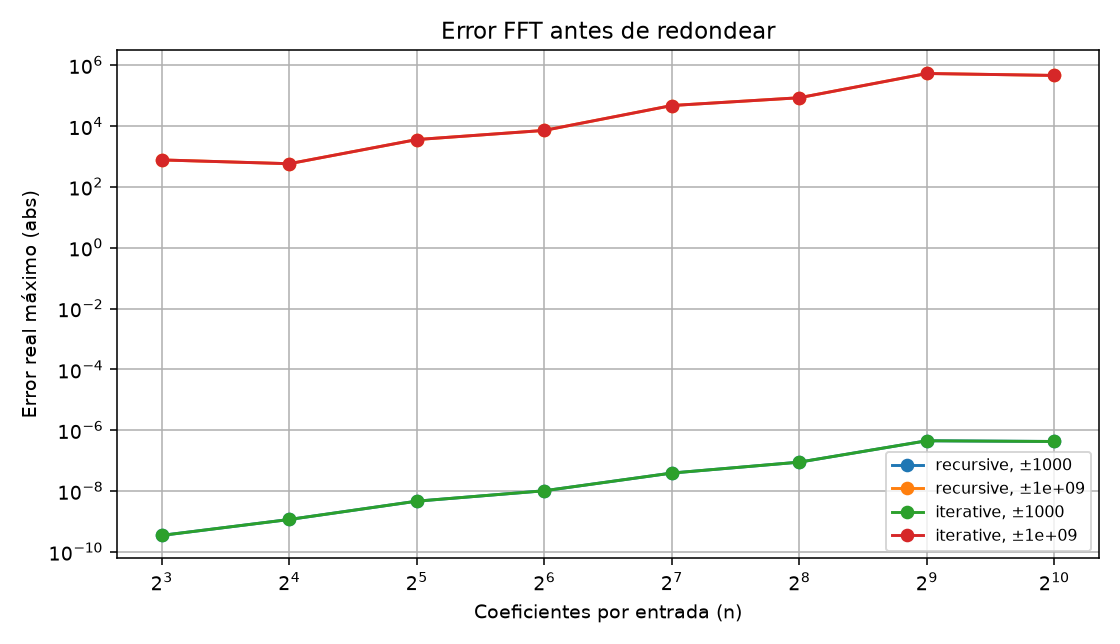
\includegraphics[width=.88\textwidth]{fig3_error_fft_vs_n.png}
\caption{Error real máximo antes del redondeo frente al tamaño $n$ para coeficientes pequeños ($[-10,10]$) y medianos ($[-1000,1000]$).}\label{fig:error}
\end{figure}

Nuestros resultados confirman que el error de punto flotante en la FFT crece de forma acotada con el tamaño $n$ y de forma proporcional al producto de las magnitudes de los coeficientes:
\begin{itemize}
    \item Para magnitudes moderadas ($\le 10^5$), el error numérico permanece estrictamente por debajo de $0.005$, garantizando un redondeo exacto al entero más cercano con cero coeficientes erróneos.
    \item Cuando los coeficientes alcanzan $10^9$ o el rango del residuo $[0, p-1]$, los coeficientes del producto exceden la capacidad de la mantisa de 53 bits del estándar IEEE 754 ($2^{53} \approx 9 \times 10^{15}$). Al superarse este umbral, los errores de redondeo se propagan a valores enteros ($\approx 4.6 \times 10^5$), generando discrepancias frente a la referencia entera.
    \item En contraste, la NTT no experimenta ninguna degradación numérica: todos los cálculos en $\mathbb{F}_p$ son rigurosamente exactos módulo $p$, consolidándose como el algoritmo idóneo para álgebra computacional de alta precisión.
\end{itemize}
